\documentclass[12pt]{article}
\usepackage[top=1in, bottom=1in, left=1in, right=1in]{geometry}

\usepackage{setspace}
\onehalfspacing

\usepackage{amssymb}
%% The amsthm package provides extended theorem environments
\usepackage{amsthm}
\usepackage{epsfig}
\usepackage{times}
\renewcommand{\ttdefault}{cmtt}
\usepackage{amsmath}
\usepackage{graphicx} % for graphics files

% Draw figures yourself
\usepackage{tikz} 

% writing elements
\usepackage{mhchem}

% The float package HAS to load before hyperref
\usepackage{float} % for psuedocode formatting
\usepackage{xspace}

% from Denovo Methods Manual
\usepackage{mathrsfs}
\usepackage[mathcal]{euscript}
\usepackage{color}
\usepackage{array}

\usepackage[pdftex]{hyperref}
\usepackage[parfill]{parskip}

% math syntax
\newcommand{\nth}{n\ensuremath{^{\text{th}}} }
\newcommand{\ve}[1]{\ensuremath{\mathbf{#1}}}
\newcommand{\Macro}{\ensuremath{\Sigma}}
\newcommand{\rvec}{\ensuremath{\vec{r}}}
\newcommand{\vecr}{\ensuremath{\vec{r}}}
\newcommand{\omvec}{\ensuremath{\hat{\Omega}}}
\newcommand{\sigs}{\ensuremath{\Sigma_s(\rvec,E'\rightarrow E,\omvec'\rightarrow\omvec)}}
\newcommand{\el}{\ensuremath{\ell}}
\newcommand{\sigso}{\ensuremath{\Sigma_{s,0}}}
\newcommand{\sigsi}{\ensuremath{\Sigma_{s,1}}}
%---------------------------------------------------------------------------
%---------------------------------------------------------------------------
\begin{document}
\begin{center}
{\bf NE 250, F15\\
September 23, 2015 
}
\end{center}

% 2013-10-01

Recall the one-group diffusion equation:

\begin{equation*}
\frac{1}{v_1}\frac{\partial \phi_1(\rvec,t)}{\partial t} = S_1(\rvec,t) - 
\Sigma_{a,1}(\rvec)\phi_1(\rvec,t) + \nabla\cdot[D_1(\rvec)\nabla\phi_1(\rvec,t)]
\end{equation*}

Now, assume that space and energy dependence of the flux can be separated:

\begin{equation*}
\phi(\vecr,E,t) = \phi(\vecr,t)\psi(E), 
\text{ where $\psi(E)$ is the neutron spectrum and $\int_0^{\infty}dE\psi(E) = 1$.}
\end{equation*}

Focusing on the spatial dependence of the flux, we'll assume a homogeneous, steady-state, one-group system.

\begin{equation*}
\frac{1}{v}\frac{\partial\phi(\rvec,t)}{\partial t} = S(\rvec,t) - \Sigma_s(\rvec)\phi(\rvec,t)
+ \nabla\cdot[D(\rvec)\nabla\phi(\rvec,t)]
\end{equation*}

Steady-state: $\frac{1}{v}\frac{\partial\phi(\rvec,t)}{\partial t} = 0$


Homogeneous: no material dependence on position; 
$\Sigma_a(\rvec)\rightarrow\Sigma_a, D(\rvec)\rightarrow D$


This gives us
%
%\begin{equation*}
%0 = S(\vecr) - \Sigma_a\phi(\vecr) + D\nabla^2\phi(\vecr)
%\end{equation*}
%
%which can be rewritten as
%
\begin{equation*}
\nabla^2\phi(\vecr) - \frac{1}{L^2}\phi(\rvec) = -\frac{S(\rvec)}{D},
\text{ where $L = \sqrt{\frac{D}{\Sigma_a}} =$ diffusion length.}
\end{equation*}

%\begin{equation*}
%L = \sqrt{\frac{\langle r^2\rangle}{6}}, \langle r^2\rangle 
%=\text{ root mean square distance from birth to absorption}
%\end{equation*}

Now, consider a plane source of strength $S_0$ in an infinitely absorbing medium.

\begin{equation*}
\phi(\rvec) = \phi(x)
\end{equation*}

\begin{equation*}
\frac{d^2\phi(x)}{dx^2} - \frac{1}{L^2}\phi(x) = -\frac{S_0\delta(x)}{D}
\end{equation*}
The boundary conditions we'd like to enforce are that the source is zero other than at the plane, so within $\epsilon \rightarrow 0$:
%
\[-D \frac{d \phi}{dx}|_{+\epsilon} + D \frac{d \phi}{dx}|_{-\epsilon} = 
J_x(0^+) - J_x(0^-) = S_0\:.\]
%
We can use this to examine two sets of equations and boundary conditions.


For $x < 0$, $\frac{d^2\phi}{dx^2} - \frac{1}{L^2}\phi(x) = 0$.

Boundary conditions: 
$\lim\limits_{x\rightarrow 0^+}\vec{J}(x) = \frac{S_0}{2}, \: \lim\limits_{x\rightarrow +\infty}|\phi(x)|<\infty, \: \phi(x) \geq 0$

For $x > 0$, \: $\frac{d^2\phi}{dx^2} - \frac{1}{L^2}\phi(x) = 0$.

Boundary conditions: 
$\lim\limits_{x\rightarrow 0^-}\vec{J}(x) = -\frac{S_0}{2}, \lim\limits_{x\rightarrow -\infty}|\phi(x)|<\infty, \phi(x) \geq 0$

With the above equations and boundary conditions, we have a general solution form of

\begin{equation*}
\phi(x) = c_1e^{-x/L} + c_2e^{x/L}.
\end{equation*}

From the finite flux condition, $c_2 = 0$. Then, $\phi(x) = c_1e^{-x/L}$.

\begin{equation*}
\lim\limits_{x\to 0^+} \vec{J}(x) = \lim\limits_{x\to 0^+}\left(\frac{D}{L}c_1e^{-x/L}\right) = 
\frac{D}{L}c_1 = \frac{S_0}{2}
\end{equation*}

\begin{equation*}
c_1 = \frac{S_0 L}{2D}
\end{equation*}

\begin{equation*}
\phi(x) = \frac{S_0L}{2D}e^{-x/L}
\end{equation*}
The neutron flux falls off exponentially as one moves away from the source plane with a characteristic decay length of $L$. This holds fairly well as long as we're not too near the source and the medium is not too strongly absorbing.

------------------------------------\\
Now, consider an infinite plane centered in a slab of finite thickness $a$, surrounded by a vacuum.


For $x > 0$, $\frac{d^2\phi}{dx^2} - \frac{1}{L^2}\phi(x) = 0$.


Boundary conditions: 
$\lim\limits_{x\rightarrow 0^+}\vec{J}(x) = \frac{S_0}{2}, \: \phi(\tfrac{\tilde{a}}{2}) = 0$

For $x < 0$, $\frac{d^2\phi}{dx^2} - \frac{1}{L^2}\phi(x) = 0$.

Boundary conditions: 
$\lim\limits_{x\rightarrow 0^-}\vec{J}(x) = -\frac{S_0}{2}, \: \phi(-\tfrac{\tilde{a}}{2}) = 0$

\begin{gather*}
\phi(x) = c_1e^{-x/L} + c_2e^{x/L} \\
\text{or (which we could have also done before)} \\
\phi(x) = c_1\cosh(\tfrac{x}{L}) + c_2\sinh(\tfrac{x}{L})
\end{gather*}
%
You can use the boundary conditions to reach the full solution.


% 2013-10-03
-------------------\\
Now, consider a uniformly distributed source of strength $S_0 \tfrac{n}{cm^3s}$ within a finite slab of
width $a$ with vacuum boundaries.

\begin{equation*}
\frac{d^2\phi(x)}{dx^2} - \frac{1}{L^2}\phi(x) = -\frac{S_0}{D}
\end{equation*}

\begin{equation*}
\phi(x) = c_1e^{-x/L} + c_2e^{x/L} + \frac{S_0L^2}{D}
\end{equation*}

Boundary conditions: $\phi(\pm\tfrac{\tilde{a}}{2}) = 0$


Alternative boundary condition: $\frac{d\phi(x)}{dx}\Bigr|_{x = 0} = 0$ (symmetry)


Now, consider a uniform source in a reflected slab, where region 2 contains the source and 1 and 3 are reflectors (high scattering compared to absorption):

\begin{center}
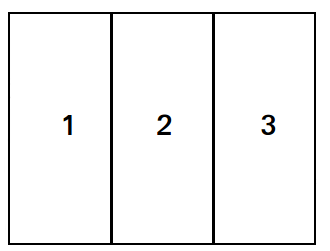
\includegraphics[height=2.5 in]{../figs/ref_slab}
\end{center}

\begin{equation*}
\frac{d^2\phi_2(x)}{dx_2^2} - \frac{1}{L_2^2}\phi_2(x) = -\frac{S_0}{D_2}, \quad -\tfrac{a}{2}<x<\tfrac{a}{2}
\end{equation*}

Boundary conditions (where subscript indicates region number):

\begin{gather*}
\phi_2(\tfrac{a}{2}) = \phi_3(\tfrac{a}{2}) \\
\vec{J}_2(\tfrac{a}{2}) = \vec{J}_3(\tfrac{a}{2}) \\
\phi_1(-\tfrac{a}{2}) = \phi_2(-\tfrac{a}{2}) \\
\vec{J}_1(-\tfrac{a}{2}) = \vec{J}_3(-\tfrac{a}{2}) 
\end{gather*}

\begin{equation*}
\frac{d^2\phi_1(x)}{dx_1^2} - \frac{1}{L_1^2}\phi_1(x) = 0, \quad -\infty<x<-\tfrac{a}{2}
\end{equation*}

\begin{equation*}
\frac{d^2\phi_3(x)}{dx_3^2} - \frac{1}{L_3^2}\phi_3(x) = 0, \quad \tfrac{a}{2}<x<\infty
\end{equation*}

Boundary conditions: 
$\lim\limits_{x\to-\infty}|\phi_1(x)| <\infty, \quad \lim\limits_{x\to\infty}|\phi_3(x)| < \infty$

----------------------\\
What if we want to solve a \textbf{generic diffusion problem}?

\begin{equation*}
D\nabla^2\phi(\rvec) - \Sigma_a\phi(\rvec) = -S(\rvec)
\end{equation*}

Working in 1D:

\begin{equation*}
M\phi(x) = f(x)
\end{equation*}
%
where $M$ is non-homogenous differential operator of order \emph{n} on a differential equation:
%
\begin{align*}
a_0(x)\phi^{(n)}(x) &+ a_1(x)\phi^{(n-1)}(x) + \dotsc + a_n(x)\phi(x) = f(x)\\
&\text{for example}\\
M = \frac{d^2}{dx^2} &- \frac{1}{L}
\end{align*}

One solution method is \textit{variation of constants / parameters}, where we break the solution into homogeneous and particular portions:
\begin{align*}
M\phi_{homog}(x) &= 0 \\
M \phi_{part} &= rhs \\
\phi(x) &= \phi_{homog}(x) + \phi_{part}(x)
\end{align*}
%
We solve the homogeneous part to yield
\[\phi_{i,h}(x),  \:i = 1,\dotsc, n \:\text{ independent solutions}\]
%
and we also know
\[\phi_{part}(x) = \sum_{i=1}^n c_i\phi_{i,h}(x)\]
%
where $c_i = c_i(x)$ and are differentiable functions that satisfy the conditions
\[\sum_{i=1}^n c'_i(x) \phi^{(j)}_{i,h}(x) = 0, \quad j = 0, \dots, n-1 \:.\]
%https://en.wikipedia.org/wiki/Variation_of_parameters

If 
\begin{align*}
\sum_{i=1}^n c_i'\phi_{i,h}(x) &= 0 \\
\sum_{i=1}^n c_i'\phi^{(1)}_{i,h}(x) &= 0 \\
&\vdots\\
\sum_{i=1}^n c_i'\phi^{(n-2)}_{i,h}(x) &= 0 \\
&\text{then} \\
\sum_{i=1}^n c_i'\phi^{(n-1)}_{i,h}(x) &= \frac{f(x)}{a_0(x)}
\end{align*}
which indicates
\begin{equation*}
c_i(x) = \int dx\:c_i'(x) \:.
\end{equation*}
%further
%\begin{align*}
%\phi_{part}(x)^{(j)} &= \sum_{i=1}^n c_i(x) \phi^{(j)}_{i,h}(x), \quad j = 0, \dots, n-1  \quad \text{and} \\
%\phi_{part}(x)^{(j)} &= \sum_{i=1}^n c_i(x) \phi^{(n)}_{i,h}(x) + \sum_{i=1}^n c'_i(x) \phi^{(n-1)}_{i,h}(x) 
%\end{align*}

For n = 2:
\vspace{-5 mm}
\begin{gather*}
\phi_1(x)c_1'(x) + \phi_2(x)c_2'(x) = 0 \\
\phi_1^{(1)}(x)c_1'(x) + \phi_2^{(1)}(x)c_2'(x) = \frac{f(x)}{a_0(x)} \\
\phi_{part} = c_1(x)\phi_1(x) + c_2(x)\phi_2(x) \\
a_0(x)\phi^{(2)}(x) + a_1(x)\phi^{(1)}(x) + a_2(x)\phi(x) = 0 \\
\phi^{(1)}(x) = c_1'(x)\phi_1(x) + c_1(x)\phi_1'(x) + c_2'(x)\phi_2(x) + c_2(x)\phi_2'(x)
\end{gather*}

\begin{equation*}
c_i(x) = \int dx c_i'(x) = A_i + \psi_i(x)
\end{equation*}

\begin{equation*}
\phi(x) = \sum_{i=1}^n A_i\phi_i(x) + \sum_{i=1}^n \psi_i(x)\phi_i(x)
\end{equation*}

For n = 2: $\phi(x) = A_1\phi_1(x) + A_2\phi_2(x) + \psi_1(x)\phi_1(x) + \psi_2(x)\phi_2(x)$


\end{document}
